\chapter{序論\label{sec:introduction}}
\thispagestyle{plain}

\section{背景}

近年,「作業通話」と呼ばれる活動が広く行われている.
作業通話とは,複数人がDiscord\cite{Discord}等の通話ツールを介して時間を共有しながら,各々の個人作業に取り組む活動を指す.
作業通話にはいくつかの別称があり,コーディングを行うエンジニアの間では「オンラインもくもく会」,イラスト制作や小説の執筆を行うクリエイターや,勉強に取り組む学生の間では「さぎょいぷ」としても浸透している.

作業通話の開催には大きく二つの利点がある.
一つ目の利点として作業効率の向上が挙げられる.
作業通話は他者と通話をしながら作業を行うことから,常に他者の存在を感じながら作業を進めることができるという特性を持つ.
それにより,個人の経験や性格によって個人差があるものの,適度に他者の存在を感じる環境にいることで観衆効果の発生が期待できる.
一般に観衆効果は作業効率が向上することが報告されている\cite{Zajonc}\cite{Matsumoto}\cite{Miyamoto}.
また,参加者同士で会話を行うことでリフレッシュ効果が期待できるほか,作業内容が類似している場合は作業中に生まれた疑問を即座に他の参加者に聞くことができるなど作業効率の向上が見込める点が多くある.
二つ目の利点として他者との関係構築の機会の増加が挙げられる.
作業通話の参加者は常に他者と通話回線がつながっており,声を発するだけで会話が始められる状態である.
また,参加者には作業を進めるという目的があることから数十分から数時間に及ぶ作業時間になることが多い.
これらの特性から自然に会話が発生し,お互いの理解が深まる.
また,並行して作業も行なっていることから無理に会話を続ける必要もなく,コミュニケーションにおける心理的な負担も小さい.
加えて,SNS上で知り合った関係が希薄もしくは皆無な人(以下,「無縁ユーザ」)と作業通話を開催する文化もあり,作業通話はコミュニケーション媒体の一種として機能している.

一方で,作業通話の参加者には各々進め方の好み(以下,「作業嗜好」)があり,それが一致する参加者を募ることが難しいという問題がある.
作業通話には開催する時間帯,作業の類似性,利用するコミュニケーションツールなどの要素があり,参加者には会話量,性格などの要素がある.
作業嗜好が合わない参加者と長時間の作業通話は,前述した作業通話の利点を十分に活かすことができない場合がある.
このことから,より効果的な作業通話の実現には作業嗜好の合う参加者を募ることが重要であるといえる.
作業通話の参加者を募る方法は大きく二つある.
一つは友人など既に所属しているコミュニティで参加者を募る方法(以下,「コミュニティ募集」)である.
コミュニティ募集は,身近な人を気軽に招待,依頼できる反面,募集対象者数が少ないため各々の都合や作業嗜好の違いによって十分に参加者が集まらない場合がある.
もう一つの募集方法として,Twitter\cite{Twitter}等のSNSを通じて不特定多数の人を対象として参加者を募る方法(以下,「SNS募集」)がある.
SNS募集は募集対象者数が多いため,その中に作業嗜好の合う人が存在する可能性が高い一方で,実際に利用されることは少ない.
これには大きく二つの要因がある.
一つ目は募集対象者が数ある募集の中からどれが自身の作業嗜好と合うものか判断することが困難であるという点である.
二つ目に募集者が無縁ユーザに対して参加者を募ることや,募集対象者が募集に対して参加意思を表明することの心理的負担が大きいという点がある.
事実,Twitter上には「作業通話したいけど勇気がでない」といった投稿が多く見られる(図\ref{fig:search_results}).

\begin{figure}
    \centering
    \fbox{
        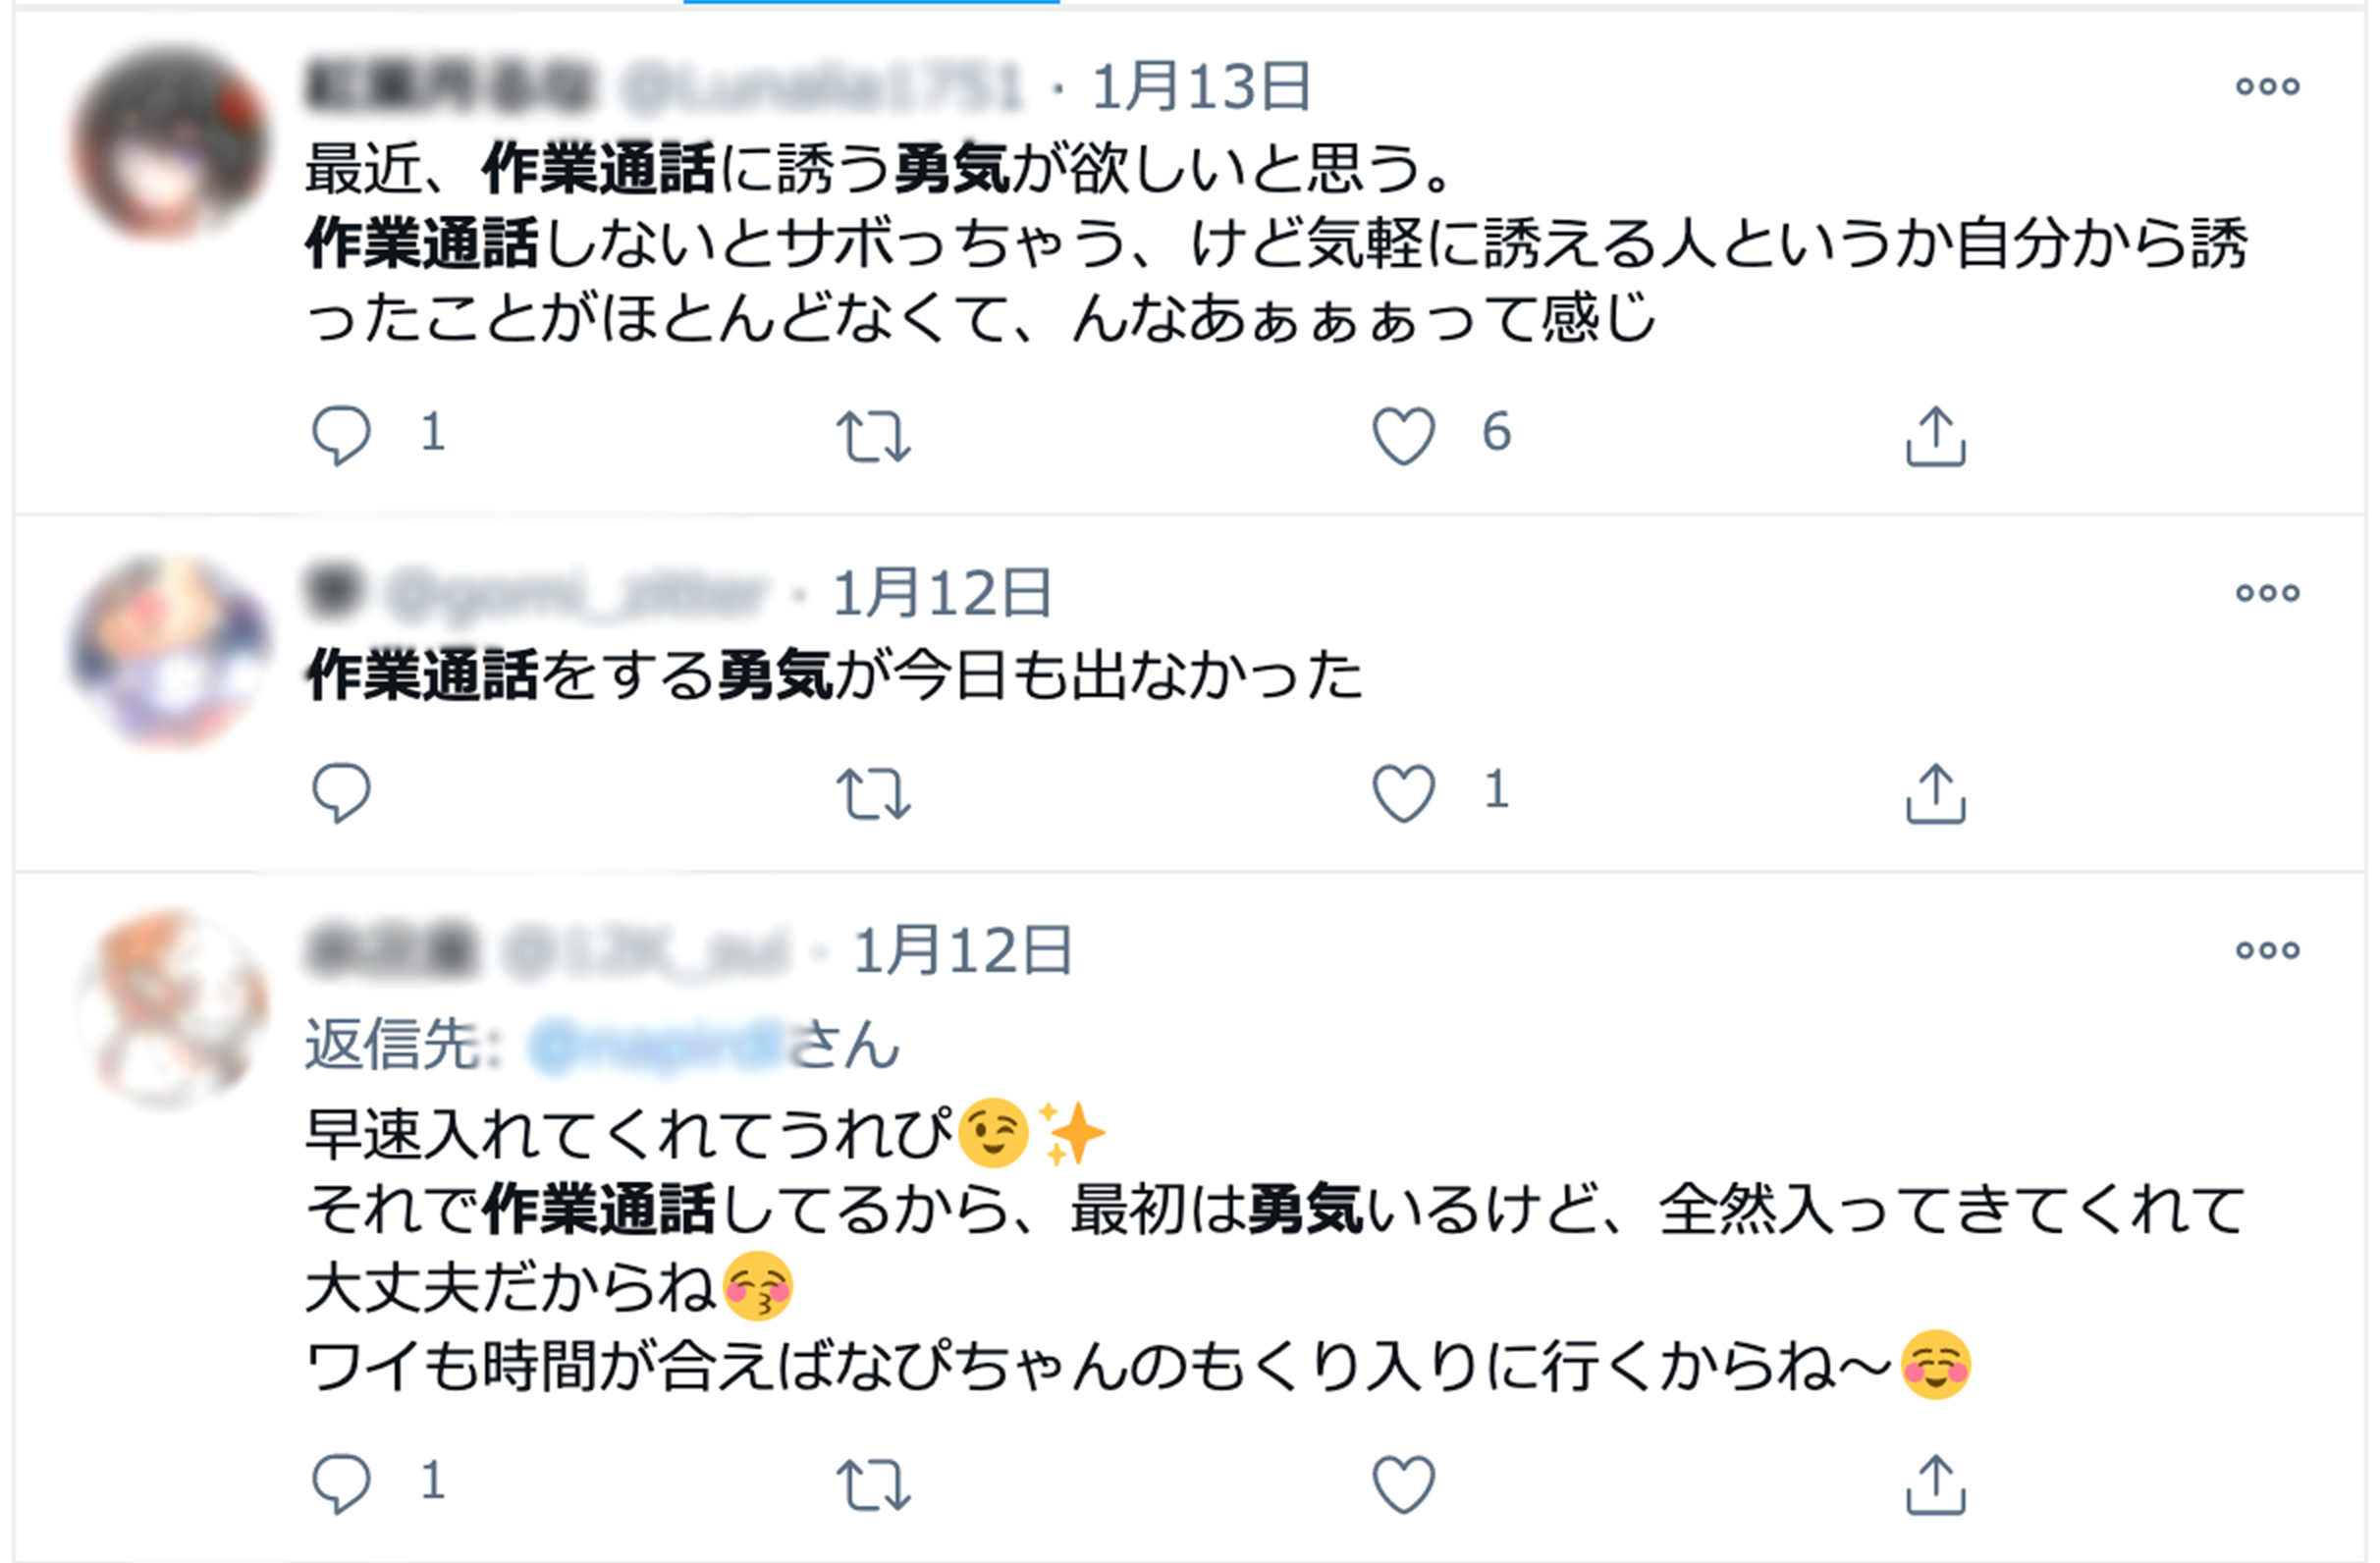
\includegraphics[width=0.7\textwidth]{figs/search_results.jpg}
    }
    \caption{Twitterで「作業通話 勇気」で検索した結果}
    \label{fig:search_results}
\end{figure}

本研究では,これら二つの要因を解消することで,作業嗜好の合う無縁ユーザとの気軽なマッチングを実現し,より効果的な作業通話の開催機会の増加を目指す.

\section{目的}

本研究の目的は,作業嗜好の合う無縁ユーザの気軽なマッチングを実現し,より効果的な作業通話の開催機会の増加を目指すことである.
そのために,作業通話の音声やメタデータから作業嗜好を推定し,可視化及び無縁ユーザのマッチングを行うシステムを提案する.
特に,本研究では対話雰囲気に着目し機械学習を用いた対話雰囲気の推定を行うことで作業嗜好の効果的な可視化を目指す.

\section{章構成}

本論文は全\ref{sec:conclusion}章で構成されている.
第\ref{sec:introduction}章では,本研究の背景と研究目的について述べた.
第\ref{sec:approach}章では,本研究のアプローチについて述べる.
第\ref{sec:related_researchs}章では,本研究に関連する研究について述べる.
第\ref{sec:proposal_system}章では,本研究で提案するシステムについて述べる.
第\ref{sec:develop_estimation_model}章では,本研究で構築した対話雰囲気推定モデルの構築について述べる.
第\ref{sec:evaluate_estimation_model}章では,本研究で構築した対話雰囲気推定モデルの評価と考察について述べる.
第\ref{sec:conclusion}章では,まとめと今後の展望について述べる.
% 第\ref{sec:evaluation_experiment}章では,評価実験について述べる.
